\sectionSlide{Birth and evolution of C++}{c++-logo}{\paperheight}

\slide{Simula}{
    Simple program in Simula
}

\slide{BCPL}{
    Before C Programming Language\\
    \pause
    Basic Combined Programming Language
}

\slide{Genealogy}{
    Genealogy of C++ from C and Simula
}

\slide{Timeline}{
    Timeline on the bottom of page, new dates will gradually appear\\
    Maybe new type of slides? TimelineSlide?
}

\slide{C with Classes}{
\begin{itemize}%[<+->]
    \item classes
    \item derived classes
    \item public and private access control
    \item constructors and destructors
    \item \textbf<2>{call and return functions (removed later)}
    \item friend classes
    \item type checking and conversion of function arguments
\end{itemize}
}

\slide{Example code in C with Classes}{
    \lstinputlisting{"src/c-with-classes.hpp"}
}

\timelineSlide{C with Classes in 1981}{
    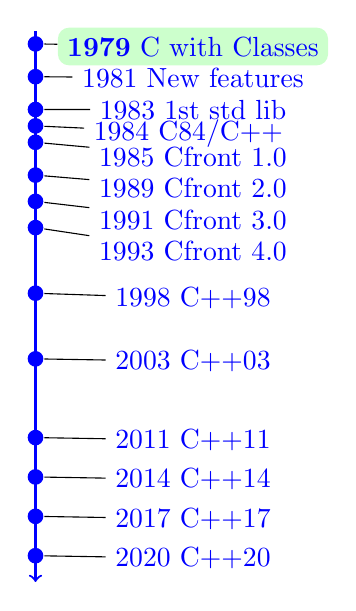
\begin{tikzpicture}
        \draw[thick,->,blue] (0,0.2)--(0,-6.8) % x axis
            node(1979)[pos=1/42,fill,circle,inner sep=2pt]{}
            node(1981)[pos=3.5/42,fill,circle,inner sep=2pt]{}
            node(1983)[pos=6/42,fill,circle,inner sep=2pt]{}
            node(1984)[pos=7.25/42,fill,circle,inner sep=2pt]{}
            node(1985)[pos=8.5/42,fill,circle,inner sep=2pt]{}
%            node(1986)[pos=8/42,fill,circle,inner sep=2pt]{}
%            node(1987)[pos=9/42,fill,circle,inner sep=2pt]{}
            node(1989)[pos=11/42,fill,circle,inner sep=2pt]{}
%            node(1990)[pos=12/42,fill,circle,inner sep=2pt]{}
            node(1991)[pos=13/42,fill,circle,inner sep=2pt]{}
            node(1993)[pos=15/42,fill,circle,inner sep=2pt]{}
            node(1998)[pos=20/42,fill,circle,inner sep=2pt]{}
            node(2003)[pos=25/42,fill,circle,inner sep=2pt]{}
            node(2011)[pos=31/42,fill,circle,inner sep=2pt]{}
            node(2014)[pos=34/42,fill,circle,inner sep=2pt]{}
            node(2017)[pos=37/42,fill,circle,inner sep=2pt]{}
            node(2020)[pos=40/42,fill,circle,inner sep=2pt]{};
            
        \draw[thin,blue]
            (2, 0) node(l1979)[fill=green!20,rounded corners] {\textbf{1979} C with Classes}
            (2,-0.4) node(l1981)[align=left] {1981 New features}
            (2,-0.8) node(l1983)[align=left] {1983 1st std lib}
            (2,-1.1) node(l1984)[align=left] {1984 C84/C++ }
            (2,-1.4) node(l1985)[align=left] {1985 Cfront 1.0}
%            (2,-2.0) node(l1986)[align=left] {1986 Cfront 1.1}
%            (2,-2.4) node(l1987)[align=left] {1987 Cfront 1.2}
            (2,-1.8) node(l1989)[align=left] {1989 Cfront 2.0}
%            (2,-3.2) node(l1990)[align=left] {1990 Cfront 2.1}
            (2,-2.2) node(l1991)[align=left] {1991 Cfront 3.0}
            (2,-2.6) node(l1993)[align=left] {1993 Cfront 4.0}
            (2,-3.2) node(l1998)[align=left] {1998 C++98}
            (2,-4.0) node(l2003)[align=left] {2003 C++03}
            (2,-5.0) node(l2011)[align=left] {2011 C++11}
            (2,-5.5) node(l2014)[align=left] {2014 C++14}
            (2,-6.0) node(l2017)[align=left] {2017 C++17}
            (2,-6.5) node(l2020)[align=left] {2020 C++20};
            
        \draw[] (1979) -- (l1979)
            (1981) -- (l1981)
            (1983) -- (l1983)
            (1984) -- (l1984)
            (1985) -- (l1985)
%            (1986) -- (l1986)
%            (1987) -- (l1987)
            (1989) -- (l1989)
%            (1990) -- (l1990)
            (1991) -- (l1991)
            (1993) -- (l1993)
            (1998) -- (l1998)
            (2003) -- (l2003)
            (2011) -- (l2011)
            (2014) -- (l2014)
            (2017) -- (l2017)
            (2020) -- (l2020)
            ;
    \end{tikzpicture}
}
{
    \begin{itemize}
        \item inline functions
        \item default arguments
        \item overloading of the assignment operator
    \end{itemize}
}

\slide{C with Classes}{
    \begin{itemize}%[<+->]
        \item classes
        \item derived classes
        \item public and private access control
        \item constructors and destructors
        \item \textbf<2>{call and return functions (removed later)}
        \item friend classes
        \item type checking and conversion of function arguments
    \end{itemize}
}
